%%%%%%%%%%%%%%%%%%%%%%%%%%%%%%%%%%%%%%%%%
% Ay 190 - WS2
% Written by Chatarin Wong-u-railertkun
%%%%%%%%%%%%%%%%%%%%%%%%%%%%%%%%%%%%%%%%%

%----------------------------------------------------------------------------------------
%	PACKAGES AND OTHER DOCUMENT CONFIGURATIONS
%----------------------------------------------------------------------------------------

\documentclass[11pt,letterpaper]{article}

% Load some basic packages that are useful to have
% and that should be part of any LaTeX installation.
%

\usepackage{graphicx}     % be able to include figures

\usepackage{xcolor}         % get nice colors

% change default font to Palatino (looks nicer!)
\usepackage[latin1]{inputenc}
\usepackage{mathpazo}
\usepackage[T1]{fontenc}

% load some useful math symbols/fonts
\usepackage{latexsym,amsfonts,amsmath,amssymb}
\usepackage{subcaption}

% comfort package to easily set margins
\usepackage[top=1in, bottom=1in, left=1in, right=1in]{geometry}

% control some spacings
%
% spacing after a paragraph
\setlength{\parskip}{.15cm}
% indentation at the top of a new paragraph
\setlength{\parindent}{0.0cm}

\usepackage{courier}


%----------------------------------------------------------------------------------------
%	TITLE
%----------------------------------------------------------------------------------------

\begin{document}

\begin{center}
\Large
Ay190 -- Worksheet 06 \\    %%%%%% DON'T FORGET TO CHANGE THE WORK SHEET NUMBER
Chatarin (Mee) Wong-u-railertkun\\
Date: \today
\end{center}

\section{Discrete Fourier Transform}

\subsection{Compare Results from \texttt{dft} and \texttt{fft}}
With the input as a vector x, \texttt{numpy.arange(10)}, table \ref{tab:compare} shows result from two methods. We can see that our method yields the result very close to those from \texttt{numpy.fft}

\begin{table}[h!]
	\centering
	\begin{tabular}{r || r | r}
		% Table Header
		Method & \texttt{dft(x)} & \texttt{fft(x)} \\
		\hline
		\hline
		%table data
		Index 0 & 45. +0.00000000e+00j & 45. +0.j \\
		Index 1 & -5. +1.53884177e+01j & -5.+15.38841769j \\
		Index 2 & -5. +6.88190960e+00j & -5. +6.8819096j \\
		Index 3 & -5. +3.63271264e+00j & -5. +3.63271264j \\
		Index 4 & -5. +1.62459848e+00j & -5. +1.62459848j \\
		Index 5 & -5. +3.53452967e-14j & -5. +0.j \\
		Index 6 & -5. -1.62459848e+00j & -5. -1.62459848j \\
		Index 7 & -5. -3.63271264e+00j & -5. -3.63271264j \\
		Index 8 & -5. -6.88190960e+00j & -5. -6.8819096j \\
		Index 9 & -5. -1.53884177e+01j & -5.-15.38841769j \\
		\hline
	\end{tabular}
	\caption{Comparing results from two methods of Fourier transform with input of (0, 1, 2, ..., 9)}
	\label{tab:compare}
\end{table}

\subsection{\texttt{dft} computational time}

From figure \ref{fig:TimeTaken}, we can see that the computational time $\propto N^{1.5}$ instead of the expected $N^2$.

\begin{figure}[h!]
	\centering
	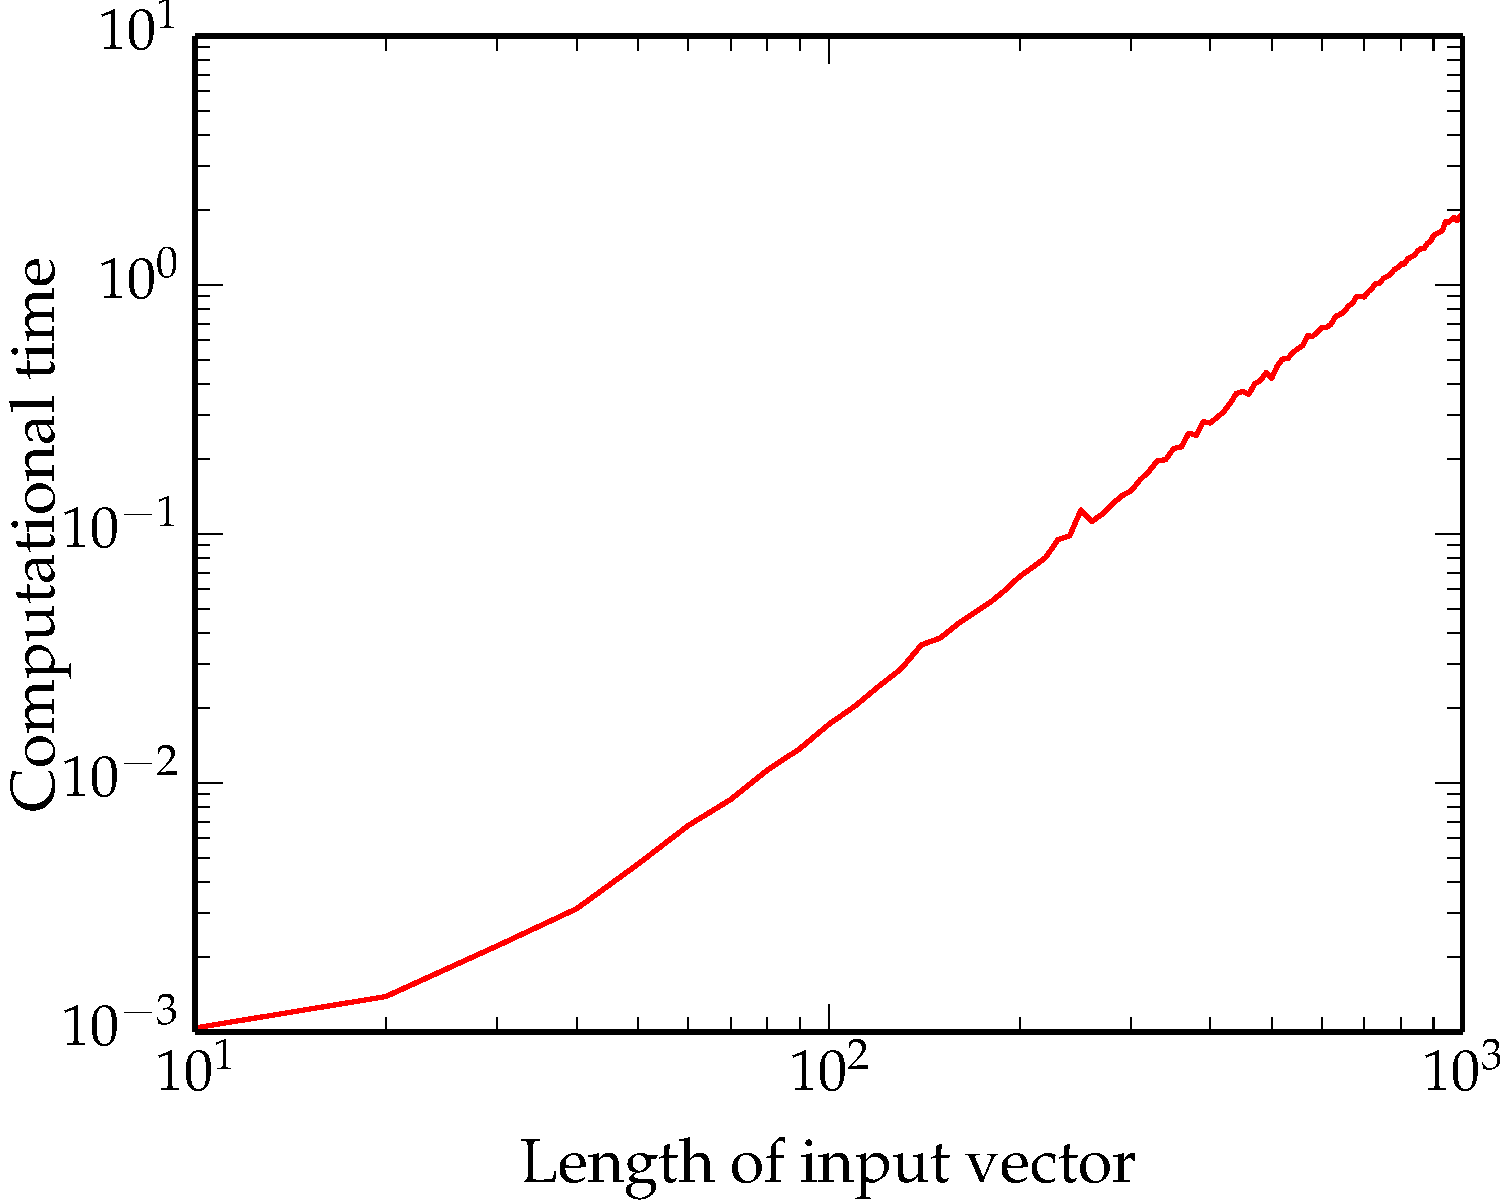
\includegraphics[width=0.5\textwidth]{TimeTaken}
	\caption{Plot the computational time of \texttt{dft} with respect to length of input vector.}
	\label{fig:TimeTaken}
\end{figure}

\subsection{Compare Computational Time}

We can see from figure \ref{fig:CompareTime} that computational time for \texttt{fft(x)} increases much slower than that of \texttt{dft(x)}.

\begin{figure}[h!]
	\centering
	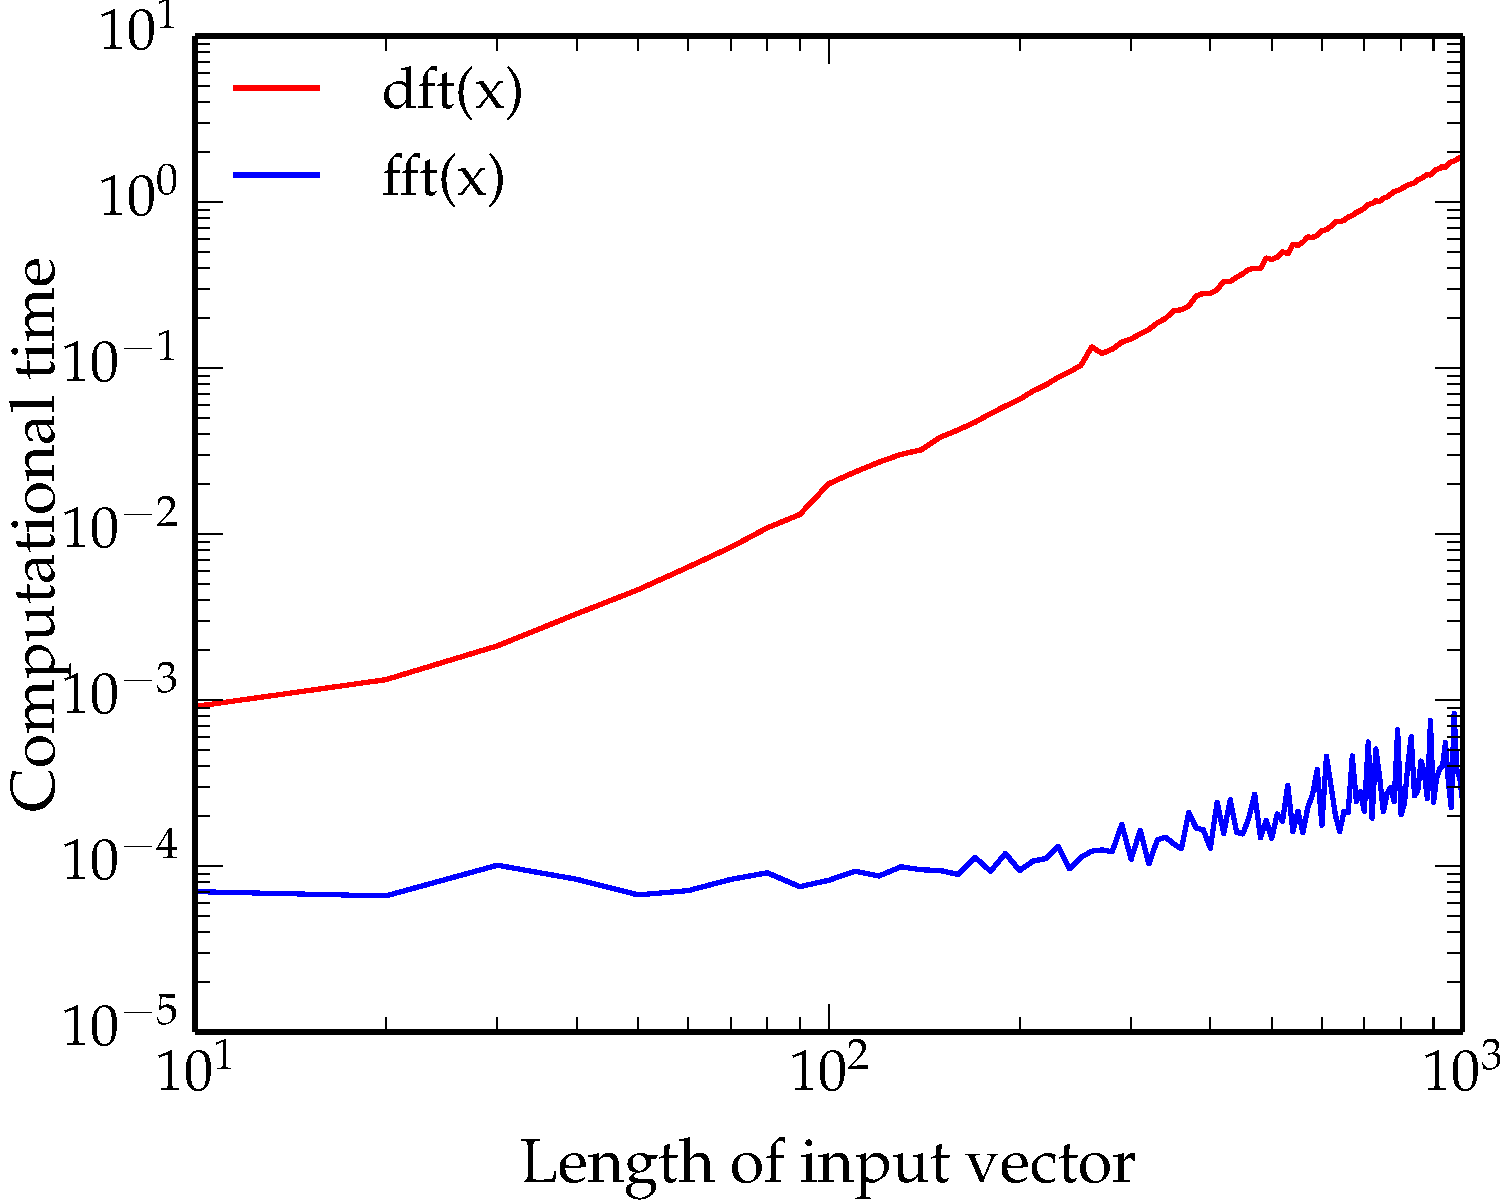
\includegraphics[width=0.5\textwidth]{CompareTime}
	\caption{Comparing the increase of computation with length of input vector, for two different methods of Fourier transform.}
	\label{fig:CompareTime}
\end{figure}

\end{document}

